% !TEX root = ../Coherence.tex


%%%%%%%%%%%%%%%%%%%%%%%%%%%%%%%%%%%%%

\subsection{Symmetric monoidal categories} 

We now formulate and prove Mac Lane's coherence theorem for \emph{symmetric} monoidal categories in the same style as above.  Recall that in a symmetric monoidal category, in addition to the natural isomorphisms $\beta$ (with components $\beta_{\kappa,\mu,\nu}:(\kappa\otimes\mu)\otimes\nu\to
\kappa\otimes(\mu\otimes\nu)$), there are natural transformations $\tau$ (with components $\tau_{\mu,\nu}:\mu\otimes\nu\to\nu\otimes\mu$. (Here, we use $\kappa,\mu,\nu,\ldots$ range over the objects of the category, consistently with the notation used in *** Sections 2.1 and 2.2 ***.)
In addition to  the pentagons (described by replacing $\circ$ with $\otimes$ in the first pentagon in~\cref{def:catoperad}), there are hexagons (for all objects $\kappa,\mu,\nu$):
\begin{center}
\resizebox{0.5\linewidth}{!}{
    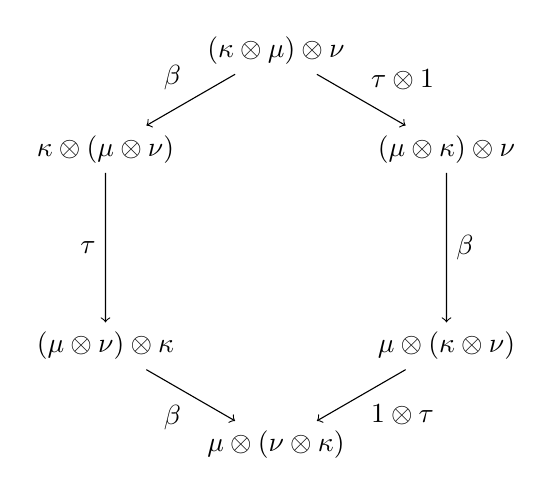
\begin{tikzpicture}[scale=2.5]
    \node (P1) at (0,1) {$(\kappa\otimes \mu) \otimes \nu$};
    \node (P2) at (-0.866,0.5) {$\kappa\otimes (\mu \otimes \nu)$};
    \node (P3) at (-0.866,-0.5) {$(\mu \otimes \nu) \otimes \kappa$};
    \node (P4) at (0,-1) {$\mu \otimes (\nu \otimes \kappa)$};
    \node (P5) at (0.866,0.5) {$(\mu \otimes \kappa) \otimes \nu$} ;
    \node (P6) at (0.866,-0.5) {$\mu \otimes (\kappa \otimes \nu)$};
    \draw[->] (P1)--(P2) node[midway,above left] {$\beta$};
    \draw[->] (P2)--(P3) node[midway,left] {$\tau$};
    \draw[->] (P3)--(P4) node[midway,below left] {$\beta$};
    \draw[->] (P1)--(P5) node[midway,above right] {$\tau\otimes 1$};
    \draw[->] (P5)--(P6) node[midway,right] {$\beta$};
    \draw[->] (P6)--(P4) node[midway,below right] {$1\otimes\tau$};
\end{tikzpicture}
}
\end{center}


We construct the free symmetric monoidal category on a set $S$.
We define a small category $\mathcal{S}^{\mathrm{ML}}$ whose set ${\cal T}_S$  is  given by the following rules:
\begin{enumerate}
    \item if $a \in S$, then $a\in{\cal T}_S$;
    \item if $t_1 \in {\cal T}_S$ and $t_2 \in {\cal T}_S$, then $t_1 \otimes t_2\in{\cal T}_S$.
\end{enumerate}
We call the elements of $S$ generating objects.

Now we define a set $M^{\mathrm{ML}}$ of basic morphisms $\beta: (t_1 \otimes t_2) \otimes t_3 \leftrightarrow t_1 \otimes (t_2\otimes t_3) : \beta^{-1}$  and $\tau: t_1\otimes t_2 \leftrightarrow t_2 \otimes t_1 : \tau^{-1}$,  for every $t_1,t_2,t_3  \in {\cal T}_S$
.
We then define the generating morphisms of  $\mathcal{S}^{\mathrm{ML}}$ by the following rules:
\begin{enumerate}
    \item if $\phi \in M^{\mathrm{ML}}$, then $\phi$ is a generating morphism; 
    \item if $\phi : t_1 \to t_2$ is a generating morphism and $t_3 \in {\cal T}_S$, then $\phi \otimes \id : t_1 \otimes t_3 \to t_2 \otimes t_3$ and $\id \otimes \phi : t_3 \otimes t_1 \to t_3 \otimes t_2$ are generating morphisms.
\end{enumerate}
We then define $\mathcal{S}^{\mathrm{ML}}$ as the free category over all generating morphisms. 
This finishes the construction of the category $\mathcal{S}^{\mathrm{ML}}$.

\begin{definition}
    We denote  by $\mathcal{F}(S)$ the quotient of $\mathcal{S}^{\mathrm{ML}}$ by localization (inverting the $\beta$ and $\tau$ morphisms), the axioms of bifunctors, the naturality conditions for $\beta$ and $\tau$, and the coherence diagrams defining   symmetric monoidal categories.
    \end{definition}

We obtain that $\mathcal{F}(S)$ is the free  symmetric monoidal category on $S$. 
That is, for any symmetric monoidal category $\mathcal{C}$, and for any function $\rho : S \to \obj(\mathcal{C})$, there is a unique \emph{strict} morphism of symmetric monoidal categories $\mathcal{F}(S) \to \mathcal{P}$ which extends $\rho$. It sends the formal basic morphisms to the actual canonical morphisms of $\mathcal{C}$.
By precomposing it with the quotient map $[-]:\mathcal{S}^{\mathrm{ML}} \to \mathcal{F}(S)$, we get  functor $\extd{-}{\mathrm{ML}}:\mathcal{S}^{\mathrm{ML}} \to \mathcal{C}$.

\smallskip
It turns out that Kapranov's topological proof is not based on the above presentation of $\mathcal{F}(S)$, but  on another presentation of this category, that is made explicit in~\cite{baralicSimplePermutoassociahedron2019}. 
We recall this presentation. We define another category $\mathcal{S}^{\mathrm{K}}$ as follows. Its objects are the same as those of $\mathcal{S}^{\mathrm{ML}}$. We define a set $M^{\mathrm{K}}$ of basic morphisms $\beta: (t_1 \otimes t_2) \otimes t_3 \leftrightarrow t_1 \otimes (t_2\otimes t_3) : \beta^{-1}$ for every $t_1,t_2,t_3  \in {\cal T}_S$ , and $\tau: a\otimes b \leftrightarrow b \otimes a : \tau^{-1}$ for every $a,b  \in S$, i.e., we \emph{limit $\tau$ to generating objects}.
Generating morphisms are defined in the same way as for $\mathcal{S}^{\mathrm{ML}}$.
We note that by construction $\mathcal{S}^{\mathrm{K}}$ is a wide subcategory of $\mathcal{S}^{\mathrm{ML}}$.

\begin{definition}
    We denote   by $\mathcal{F}(S)^{\mathrm{K}}$ the quotient of $\mathcal{S}^{\mathrm{K}}$ by localization (inverting the $\beta$ and $\tau$ morphisms), the axioms of bifunctors, the naturality conditions for $\beta$, and the coherence diagrams defining   monoidal categories  and by the  axioms in dodecagonal form (for $a,b,c$ ranging on $S$ only) given by the solid arrows in~\cref{fig:dodecagon}.
\end{definition}
\begin{figure}[h!]
\begin{center}
\resizebox{0.8\linewidth}{!}{
 \begin{tikzpicture}[scale=6.5]
    \node (P1) at (0,1) {$(a \otimes b) \otimes c$};
    \node (P2) at (-0.5,0.866) {$a \otimes (b \otimes c)$};
    \node (P3) at (-0.866,0.5) {$a \otimes (c \otimes b)$};
    \node (P4) at (-1,0) {$(a \otimes c) \otimes b$};
    \node (P5) at (-0.866,-0.5) {$(c \otimes a) \otimes b$} ;
    \node (P6) at (-0.5,-0.866) {$c \otimes (a \otimes b)$};
    \node (P7) at (0,-1) {$c \otimes (b \otimes a)$};
    \node (P8) at (0.5,-0.866) {$(c \otimes b) \otimes a$};
    \node (P9) at (0.866,-0.5) {$(b \otimes c) \otimes a$};
    \node (P10) at (1,0) {$b \otimes (c \otimes a)$};
    \node (P11) at (0.866,0.5) {$b \otimes (a \otimes c)$} ;
    \node (P12) at (0.5,0.866) {$(b \otimes a) \otimes c$};
    \draw[->] (P1)--(P2) node[midway,above left] {$\beta$};
    \draw[->] (P2)--(P3) node[midway,above left] {$1\otimes\tau$};
    \draw[->] (P3)--(P4) node[midway,above left] {$\beta^{-1}$};
    \draw[->] (P4)--(P5) node[midway,below left] {$\tau\otimes 1$};
    \draw[->] (P5)--(P6) node[midway,below left] {$\beta$};
    \draw[->] (P6)--(P7) node[midway,below left] {$1\otimes\tau$};
    \draw[->] (P1)--(P12) node[midway,above right] {$\tau\otimes 1$};
    \draw[->] (P12)--(P11) node[midway,above right] {$\beta$};
    \draw[->] (P11)--(P10) node[midway,above right] {$1\otimes\tau$};
    \draw[->] (P10)--(P9) node[midway,below right] {$\beta^{-1}$};
    \draw[->] (P9)--(P8) node[midway,below right] {$\tau\otimes 1$};
    \draw[->] (P8)--(P7) node[midway,below right] {$\beta$};
    \draw[->,dashed] (P2)--(P9) node[midway,above right] {$\tau$};
    \draw[->,dashed] (P3)--(P8) node[midway,below left] {$\tau$};
\end{tikzpicture}
\quad\quad
 \begin{tikzpicture}[scale=6.5]
    \node (P1) at (0,1) {$(\set{a}  \set{b})  \set{c}$};
    \node (P2) at (-0.5,0.866) {$\set{a}  (\set{b}  \set{c})$};
    \node (P3) at (-0.866,0.5) {$\set{a}  (\set{c}  \set{b})$};
    \node (P4) at (-1,0) {$(\set{a}  \set{c})  \set{b}$};
    \node (P5) at (-0.866,-0.5) {$(\set{c}  \set{a})  \set{b}$} ;
    \node (P6) at (-0.5,-0.866) {$\set{c}  (\set{a}  \set{b})$};
    \node (P7) at (0,-1) {$\set{c}  (\set{b}  \set{a})$};
    \node (P8) at (0.5,-0.866) {$(\set{c}  \set{b})  \set{a}$};
    \node (P9) at (0.866,-0.5) {$(\set{b}  \set{c})  \set{a}$};
    \node (P10) at (1,0) {$\set{b}  (\set{c}  \set{a})$};
    \node (P11) at (0.866,0.5) {$\set{b}  (\set{a}  \set{c})$} ;
    \node (P12) at (0.5,0.866) {$(\set{b}  \set{a})  \set{c}$};
    \node (P13) at (0,0) {$\set{a,b,c}$} ;
    \draw[-] (P1)--(P2) node[midway,above left] {$\set{a}\set{b}\set{c}$};
    \draw[-] (P2)--(P3) node[midway,above left] {$\set{a}\set{b,c}$};
    \draw[-] (P3)--(P4) node[midway,above left] {$\set{a}\set{c}\set{b}$};
    \draw[-] (P4)--(P5) node[midway,below left] {$\set{a,c}\set{b}$};
    \draw[-] (P5)--(P6) node[midway,below left] {$\set{c}\set{a}\set{b}$};
    \draw[-] (P6)--(P7) node[midway,below left] {$\set{c}\set{a,b}$};
    \draw[-] (P1)--(P12) node[midway,above right] {$\set{a,b}\set{c}$};
    \draw[-] (P12)--(P11) node[midway,above right] {$\set{b}\set{a}\set{c}$};
    \draw[-] (P11)--(P10) node[midway,above right] {$\set{b}\set{a,c}$};
    \draw[-] (P10)--(P9) node[midway,below right] {$\set{b}\set{c}\set{a}$};
    \draw[-] (P9)--(P8) node[midway,below right] {$\set{b,c}\set{a}$};
    \draw[-] (P8)--(P7) node[midway,below right] {$\set{c}\set{b}\set{a}$};
\end{tikzpicture}} 

\end{center}
\caption{Kapranov dodecagons}
\label{fig:dodecagon}
\end{figure}

We pause here to reflect on the difference between the two presentations. In the second, we have less generators, and we have lost hexagons. For an intuition, here is how Mac Lane himself motivated his hexagonal axioms (verbatim, just changing the notation to fit with ours) in~\cite{MacLane63}:

\begin{quote}
The instance $\tau_{\kappa\otimes \mu,\nu}$ interchanges the block $\kappa\mu$ with the single letter $\nu$; the hexagon condition states that this interchange may be replaced by two instances of $\tau$ which interchange single letters with $\nu$. Repeated such replacement using instances of the hexagon shows that any interchange of successive blocks may be replaced by interchanges of successive letters.
\end{quote}

In other words, hexagons are now taken as definitions rather than axioms. But how do we guarantee that the  general $\tau$ morphisms defined in this way define a natural transformation? This is what the dodecagons are for, as we shall see.

\smallskip
Let $\mathcal{C}$  be a symmetric monoidal category. Then by freeness  $\rho : S \to \obj(\mathcal{C})$, $\rho$ extends uniquely to a functor $\extd{-}{\mathrm{K}}:\mathcal{S}^{\mathrm{K}} \to \mathcal{C}$.
This functor is the restriction of $\extd{-}{\mathrm{ML}}$ to $\mathcal{S}^{\mathrm{K}}$.
In the next proposition, we  establish ``Kapranov style'' coherence.



\begin{proposition}
\label{thm:coherence-Kapranov}
    For any symmetric monoidal category $\mathcal{C}$, for any  function $\rho : S \to \obj(\mathcal{C})$, and for any two parallel morphisms $\phi_1,\phi_2: t_1 \to t_2$ in~$\mathcal{S}^{\mathrm{K}}$, we have $\extd{\phi_1}{\mathrm{K}}=\extd{\phi_2}{\mathrm{K}}$.
\end{proposition}
\begin{proof}
The conclusion will readily follow from the following two properties
\begin{enumerate}
\item[(1)] If $\phi_1,\phi_2: t_1 \to t_2$ in~$\mathcal{S}^{\mathrm{K}}$, then $[\phi_1]^{\mathrm{K}}=[\phi_2]^{\mathrm{K}}$, where $[-]^{\mathrm{K}}:\mathcal{S}^{\mathrm{K}}\to  \mathcal{F}(S)^{\mathrm{K}}$ is the quotient functor.  
\item[(2)] The relations in Kapranov presentation are valid in $\mathcal C$.
\end{enumerate} 
Indeed, (2) says that $\extd{-}{\mathrm{K}}$ factors through $[-]^{\mathrm{K}}$, hence the statement is reduced to proving (1).

The proof of  (2) is visualised in~\cref{fig:dodecagon} (left part).  The two dotted lines delimit two Mac Lane hexagons on the top and at the bottom and a naturality square in the middle (explicitly, the two dotted $\tau$ morphisms are $\tau_{a,b\otimes c}$ and $\tau_{a,c\otimes b}$. 

 We prove (1) as an application of our general theory of~\cref{s:polycoherence}, like in the categorified operadic case. Again, we  exhibit  a bijective correspondence between the $i$-dimensional faces of Kapranov's poset ${\mathcal P}$ (realised later as a polytope in~\cite{reinerCoxeterassociahedra1994}), for $0\leq i\leq 2$, and the data defining $\mathcal{S}^{\mathrm{K}}$.  We start by presenting this poset. We fix a finite  subset $A\inc S$ of generating objects. 
 An element of $P$ is a (non necessarily fully) parenthesised word whose letters are finite non-empty subsets of $A$ forming a partition of $A$.  For example, with $A=\set{a_1,\ldots,a_6,a_7}$, the following is a face:
 $$\begin{array}{l}
 (\set{a_1} \set{a_4} \set{a_2,a_6}) \set{a_3,a_5,a_7}
 \end{array}$$
The elements of $P$ can be drawn as planar trees whose leaves are decorated with subsets of $A$ forming together a partition of $A$.  The subface relation $\prec$ is defined by two clauses: one can contract an edge of the tree (or remove a node all of whose  incoming edges are leaves and decorate its outcoming edge -- now a leaf- with the union of the decorations of those incoming edges, as illustrated below:
$$\begin{array}{lll}
 (\set{a_1} \set{a_4} \set{a_2,a_6}) \set{a_3,a_5,a_7} & \prec & \set{a_1} \set{a_4} \set{a_2,a_6} \set{a_3,a_5,a_7} \\
 (\set{a_1} \set{a_4} \set{a_2,a_6}) \set{a_3,a_5,a_7} & \prec &  \set{a_1,a_2,a_4,a_6} \set{a_3,a_5,a_7}
 \end{array}$$
 The maximum face is $A$.
These posets, parametrized by $A$, have been realized by CW-complexes (resp. by polytopes) in \cite{kapranov1993} (resp. \cite{reinerCoxeterassociahedra1994}).
The 0-dimensional faces of $P$ are fully parenthesized words whose letters are singletons, and are in obvious bijective correspondence with the elements of ${\cal T}_A$ in which each generating object occurs exactly once (as in all coherence conditions).  The 1-dimensional faces are 
\begin{itemize}
\item
either fully parenthesised words whose letters are singletons but for one letter which is a two element set $\set{a_i,a_j}$ and feature a generating morphism whose underlying basic morphism is $\tau_{a_i,a_j}$, 
\item or an ``almost'' fully parenthesised word of singletons, with just one parenthesis removed, yielding a subword $\set{a_i,a_j,a_k}$, featuring an application of the basic morphism $\beta_{a_i,a_j,a_k}$ or $\beta_{a_i,a_j,a_k}^{-1}$
-- the orientation being ``decided'' by	 the shape of the end vertices.
\end{itemize}
Finally, the 2-dimensional faces can be analysed much in the same way as in  ***Proposition 2.6 ***, and seen to correspond to bifunctoriality, naturality of $\beta$, and to the pentagons and dodecagons. We have picture the poset view of the 
latter in~\cref{fig:dodecagon} (right part).
\end{proof}

The following proposition seems unrelated to coherence issues, but in fact its proof relies on the  coherence result that we just established.
\begin{proposition} \label{Kapranov-MacLane}
The identity-on-objects  functor from  $\mathcal{F}(S)^{\mathrm{K}}$ to 
$\mathcal{F}(S)$ that maps $[\psi]^{\mathrm{K}}$ to $[\psi]$ is an isomorphism of categories.
\end{proposition}

\begin{proof}
We first note that it follows from (2) in the proof of~\cref{thm:coherence-Kapranov} (applied to $\mathcal{F}(S)$) that the map in the statement is well defined. We build a map in the converse direction.
 For each morphism $\phi\in\mathcal{S}^{\mathrm{ML}}$, there exists a morphism $\psi\in\mathcal{S}^{\mathrm{K}}$ such that $[\phi]=[\psi]$. Such a morphism can be obtained by repeatedly applying the procedure described in the above quotation of Mac Lane.  We define a candidate for being an inverse of the map in the statement by mapping $[\phi]$ to $[\psi]^{\mathrm{K}}$. We show that this  map is well-defined. Indeed, if  a morphism $\phi'$ of  $\mathcal{S}^{\mathrm{ML}}$ is such that $[\phi]=[\phi']$ and if $\psi'$ is a morphism of $\mathcal{S}^{\mathrm{K}}$ such that $[\phi]=[\psi']$, then a fortiori $\psi$ and $\psi'$ are parallel, and hence by (1) in the proof of~\cref{thm:coherence-Kapranov}, we get  $[\psi]^{\mathrm{K}}=[\psi']^{\mathrm{K}}$. 
 Finally, starting from  $[\phi]\in\mathcal{F}(S)$, applying the two maps successively returns  $[\psi]$ which is equal to $[\phi]$ by construction. In the other direction, starting from $[\psi]^{\mathrm{K}}$, we get $[\psi]$ and  we have nothing to do to pick a representative from $\mathcal{S}^{\mathrm{K}}$, so that applying the two maps does nothing either.
\end{proof}

\begin{thm}[Coherence theorem]
\label{thm:coherence-MacLane}
    For any symmetric monoidal category $\mathcal{C}$, for any  function $\rho : S \to \obj(\mathcal{C})$, and for any two parallel morphisms $\phi_1,\phi_2: t_1 \to t_2$ in~$\mathcal{S}^{\mathrm{ML}}$, we have $\extd{\phi_1}{\mathrm{ML}}=\extd{\phi_2}{\mathrm{ML}}$.
\end{thm}
\begin{proof} 
If $\phi_1$ and $\phi_2$ are parallel in $\mathcal{S}^{\mathrm{ML}}$, then by~\cref{Kapranov-MacLane}
there exist $\psi_1$ and $\psi_2$ in $\mathcal{S}^{\mathrm{K}}$ such that $[\psi_1]=[\phi_1]$ and 
$[\psi_2]=[\phi_2]$
 (in particular $\psi_1$ and $\psi_2$ are parallel).
Then we have  
$$\extd{\phi_1}{\mathrm{ML}} = \extd{\psi_1}{\mathrm{ML}}= \extd{\psi_1}{\mathrm{K}} 
=  \extd{\psi_2}{\mathrm{K}} 
 =  \extd{\psi_2}{\mathrm{ML}}  =  \extd{\phi_2}{\mathrm{ML}}$$ 
 where the equality in the middle 
follows from~\cref{thm:coherence-Kapranov}.
\end{proof}

%{\color{blue} OBSOLETE
%One can use the same ideas to prove MacLane's coherence theorem for \emph{symmetric} monoidal categories, using the family of permutoassociahedra \cite{kapranov1993,reinerCoxeterassociahedra1994,baralicSimplePermutoassociahedron2019,CastilloLiu21}. 
%Here we simply formulate the theorem, the proof is really the same as the one of \cref{thm:coherence-operahedra}.
%
%Let $W_n$ denote the set of non-commutative, fully parenthesized words on $n$ distinct letters. 
%Let $(\mathcal{C}, \otimes)$ be a symmetric monoidal category.
%Each $w \in W_n$ defines in an obvious way a functor $[w] : \mathcal{C}^{\times n} \to \mathcal{C}$.
%For instance, if $w=((ab)c)(ed)$, then the associated functor is defined on objects and morphisms by the formula
%\begin{eqnarray*}
%    [w] \quad : \quad \mathcal{C}^{\times n} & \to & \mathcal{C} \\
%    (a,b,c,d,e) & \mapsto & ((a \otimes b) \otimes c)\otimes (e \otimes d) \ .
%\end{eqnarray*}
%We consider the free category $\mathcal{W}_n$ which has objects the elements of $W_n$, and morphisms generated by the ones of the form $\phi : w_1 \to w_2$, where the word $w_2$ is obtained from $w_1$ by applying either $\alpha : ((ww')w'') \to (w(w'w''))$, $\alpha^{-1}$, or $\tau : ww' \to w'w$ to a subword of $w_1$.
%To any such $\phi$ one can associate a natural transformation $[\phi] : [w_1] \to [w_2]$ in $\mathcal{C}$ in the obvious way. 
%
%\begin{thm}[MacLane's coherence theorem]
%    \label{thm:MacLanesym}
%    For any symmetric monoidal category $\mathcal{C}$, and for any pair of parallel morphisms $\phi_1,\phi_2: w_1 \to w_2$ in $\mathcal{W}=\{\mathcal{W}_n\}_{n\geq 1}$, we have $[\phi_1]=[\phi_2]$.
%\end{thm}}










%\begin{rem}
%\label{rem:29}
%MacLane's original proof \cite{MacLane63} proceeds in two stages, (anachronically) much like the one of Do{\v s}en--Petri{\'c} for weak Cat-operads (\cref{rem:DPLA}).
%But the second proof of \cref{thm:coherence-operahedra} suggests a one stage proof: indeed, fixing a total order on the letters, allowing $\tau: ab \to ba$ only if the maximal letter is in $a$ (and adding $\tau^{-1}$), we get a terminating and confluent rewriting system. 
%\end{rem}

